\chapter{Simulation}
This chapter discusses some simulation results, using a simple mathematical model to create a controller. First the mathematical model is discussed, after that the simulation results are discussed and compared with the internal Matlab solvers.

\section{Trailer model}
The trailer model is illustrated in figure~\ref{fig:trailer model}, the left rectangle is the trailer and the right rectangle is the driver. The driver pulls the trailer forward. The driver is connect to the trailer via a single arm as illustrated in figure~\ref{fig:trailer model}. The control system can only change the speed in the Y and X axis. The goal of the control system is to get the trailer at a certain position and at a certain angle. Figure shows the trailer in a neutral position, so under an angle of 0 degrees.

\begin{figure}
	\centering
	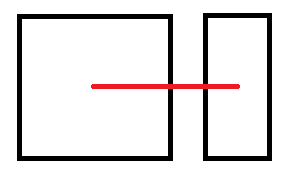
\includegraphics[width=0.5\textwidth]{trailer}
	\caption{trailer}
	\label{fig:trailer model}
\end{figure}

The mathematical model of the trailer is represented in equation~\ref{eq:trailer model}, $u_x$ and $u_y$ are the inputs of the system and represent the speed in the Y and X direction. The angle is represented by $\theta$ , the distance between the driver and the trailer is represented by L. The position of the trailer is represented by $p_x$ and $p_y$.

\begin{equation}
	\begin{cases}
		\dot{p_x} = u_x + L sin \theta \cdot \dot{\theta} \\
		\dot{p_y} = u_y + L cos \theta \cdot \dot{\theta} \\
		\dot{\theta} = \frac{1}{L}(u_ycos \theta - u_x sin \theta)	
	\end{cases}
	\label{eq:trailer model}
\end{equation}

\section{A simple trailer example}
A simple way of measuring the performance of the library is to compared it to the alternatives. In the following simulation the nmpc-codegen library will be compared to, ForBes zerofrp2 the Matlab implementation of the panoc algorithm. And to the internal Matlab function fmincon using either of the tree algorithms interior point,SQP and active set.

The simulation will contain four circular obstacles and the trailer will move from the lower left corner to the upper right corner. Each of the algorithms will calculate the optimum path up to the tolerance of $10^{-3}$. The input for one step is then applied to the system equation, and the next state is obtained. The same nmpc problem is solved using the new state as current state  and the new input is applied again.

The state of the trailer will is represented by arrows, the starting point of the arrow is the position of the trailer. The angle of the arrow represents the positional angle of the trailer. The amplitude of the arrow has no meaning.

Figure~\ref{fig:solution path trailer example} contains the results of the simulation. The panoc algorithm calculated the lowest located path while all three of the fmincon algorithms opted for the upper located path. Both of these paths are valid solutions. It is immediately clear from figure~\ref{fig:timings trailer example} that the nmpc-codegen library is significantly faster. The other four algorithm's are about the same for the first 30 steps, after about 30 steps the ForBes zerofpr2 algorithm is faster then either of the tree fmincon algorithms.

The nmpc-codegen library uses a cautious lbfgs update which improves the performance of the lbfgs. This is clear from figure~\ref{fig:iterations trailer example} where not the time to convergence but iterations till convergence are illustrated. The nmpc-codegen clearly needs less iterations than theForbes zerofpr2. As the simulation progresses, less and less iterations are needed to calculate optimal solution. And the lbfgs doesn't influence the convergence as much, so the two algorithms have about the same amount iterations till convergence.
\begin{figure}[H]
	\centering
	\begin{subfigure}[b]{0.45\textwidth}
		\centering
		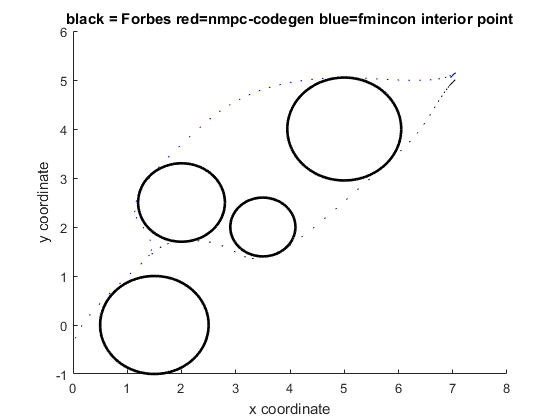
\includegraphics[width=1.2\textwidth]{compare_libs/path}
		\caption{path}
		\label{fig:solution path trailer example}
	\end{subfigure}
	
	\begin{subfigure}[b]{0.45\textwidth}
		\centering
		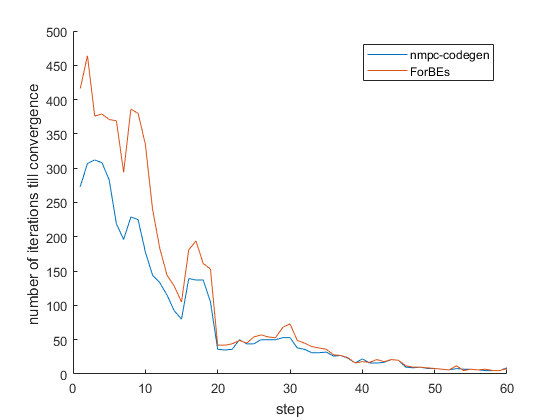
\includegraphics[width=1.2\textwidth]{compare_libs/iterations}
		\caption{iterations}
		\label{fig:iterations trailer example}
	\end{subfigure}
	\hfill
	\begin{subfigure}[b]{0.45\textwidth}
		\centering
		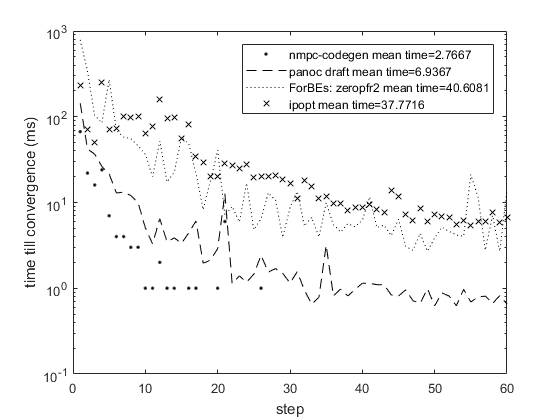
\includegraphics[width=1.2\textwidth]{compare_libs/timings}
		\caption{timings}
		\label{fig:timings trailer example}
	\end{subfigure}
	\caption{Schematic representation of the software}
\end{figure}

\section{Conclusion}

The simulations clearly indicate that a great speed up his gained by implementing the panoc algorithm in C. As the algorithm doesn't require a lot of memory it can be run efficiently on small embedded devices. The control engineer can design and test the performance of the algorithm in either Matlab or Python.